\clearpage
\section{Extension study E1--E3}\label{app:extension}
\paragraph{Design and freeze.} The extension was specified after the core results showed that S2 stalled. It was frozen in \path{code/simulation/results/extension/extension-design.json} before any extension mission was run. The core design hash is recorded inside it. Pilot seeds 0--9 supplied all selections. Margins were chosen from $\{0,2,4\}$ dB, EWMA $\alpha\in\{0.3,0.6\}$, Kalman $q\in\{10^{-3},10^{-2}\}$ and $r\in\{1,25\}$, and Gilbert $\tau\in\{0.1,0.2,0.3,0.5\}$. Learned thresholds were chosen from $\{0.1,\dots,0.9\}$. The selected values were 4 dB for trend, persistence, EWMA ($\alpha=0.3$) and Kalman ($q=10^{-3}$, $r=1$); $\tau=0.1$ with 0 dB for Gilbert; 0.5 for both learned models; and 0 dB for the oracle.

The Gilbert transition probabilities ($p_{CF}=0.062$, $p_{FC}=0.286$) were pooled from the pilot fade sequences, which acted as a labelled calibration campaign. Along fixed routes a faded exchange almost never succeeds, so the fade state cannot be learned from successful samples alone. A first freeze that tried to do so produced zero transitions. It was discarded before any evaluation outcome was inspected; the repository work log records this.

Learned features are nine causal quantities from successful samples: the current margin to the threshold, four motion-projected signals, the residual, its slope, the sampling gap and the range rate. Positive labels mark a successful sample followed by an eligible onset within 1--3 exchanges (9.6\% of 4693 training rows). Both models were trained in NumPy, with class-balanced weights, L2 regularisation and fixed seeds.

\begin{table}[htbp]\centering\small
\caption{Held-out fixed-route warning quality (extension seeds 2000--2029, 180 traces) with per-decision counted work and retained binary64 state. Ops are counted arithmetic; transcendental calls are logarithms, square roots, exponentials and tanh. The oracle is not deployable.}\label{tab:predictors}
\begin{tabular}{lrrrrrrr}\toprule
Predictor & Prec. & Recall & F1 & Lead [s] & Ops/dec. & Transc./dec. & Memory [B]\\\midrule
Trend (frozen) & 0.15 & 0.27 & 0.192 & 18.9 & 136 & 12.5 & 208\\
Persistence (frozen) & 0.15 & 0.27 & 0.193 & 18.9 & 1 & 0.0 & 16\\
EWMA residual & 0.15 & 0.27 & 0.192 & 18.9 & 61 & 9.0 & 64\\
Kalman level/slope & 0.15 & 0.27 & 0.192 & 18.9 & 102 & 9.0 & 120\\
Gilbert burst HMM & 0.15 & 0.27 & 0.193 & 18.9 & 266 & 9.0 & 216\\
Logistic regression & 0.14 & 0.09 & 0.106 & 20.0 & 117 & 11.0 & 272\\
MLP (16 tanh) & 0.15 & 0.24 & 0.185 & 18.6 & 419 & 27.0 & 1736\\
Fade oracle (bound) & 0.75 & 0.98 & 0.850 & 27.5 & 53 & 8.0 & 8\\
\bottomrule\end{tabular}

\end{table}

\paragraph{Recovery rule.} The meeting cells are the two adjacent cells $(9,6)$ and $(10,6)$. Recovery affects only online policies, and S1 runs are identical with and without it. Recovery travel observes cells like any other motion, so it can add redundant observations. The extension's primary contrast remains S4-T minus S2; S4-T minus S3 and S4-T minus S4-P are secondary. Each further predictor is compared with S3 and S2.

\begin{table}[htbp]\centering\scriptsize
\caption{Extension restricted mean time [s] per condition (30 seeds each) and completions out of 180. All extension missions completed.}
\resizebox{\linewidth}{!}{\begin{tabular}{llrrrrrrrrrrr}\toprule
Progress & $L$ & S1 & S2 & S3 & S4-T & S4-P & S4-E & S4-K & S4-G & S4-L & S4-M & S4-O\\\midrule
Balanced & 2 & 1280 & 1544 & 1422 & 1435 & 1432 & 1428 & 1432 & 1422 & 1433 & 1452 & 1424\\
Balanced & 5 & 1280 & 1643 & 1459 & 1484 & 1486 & 1484 & 1484 & 1459 & 1471 & 1515 & 1459\\
Balanced & 10 & 1280 & 1614 & 1433 & 1446 & 1464 & 1445 & 1446 & 1433 & 1450 & 1485 & 1436\\
Unequal & 2 & 1423 & 1627 & 1493 & 1516 & 1517 & 1509 & 1515 & 1500 & 1512 & 1516 & 1502\\
Unequal & 5 & 1423 & 1711 & 1512 & 1541 & 1547 & 1538 & 1540 & 1516 & 1522 & 1589 & 1523\\
Unequal & 10 & 1423 & 1708 & 1507 & 1534 & 1550 & 1533 & 1534 & 1517 & 1536 & 1557 & 1521\\
\midrule
Completed & all & 180 & 180 & 180 & 180 & 180 & 180 & 180 & 180 & 180 & 180 & 180\\
\bottomrule\end{tabular}
}
\end{table}
\begin{figure}[htbp]\centering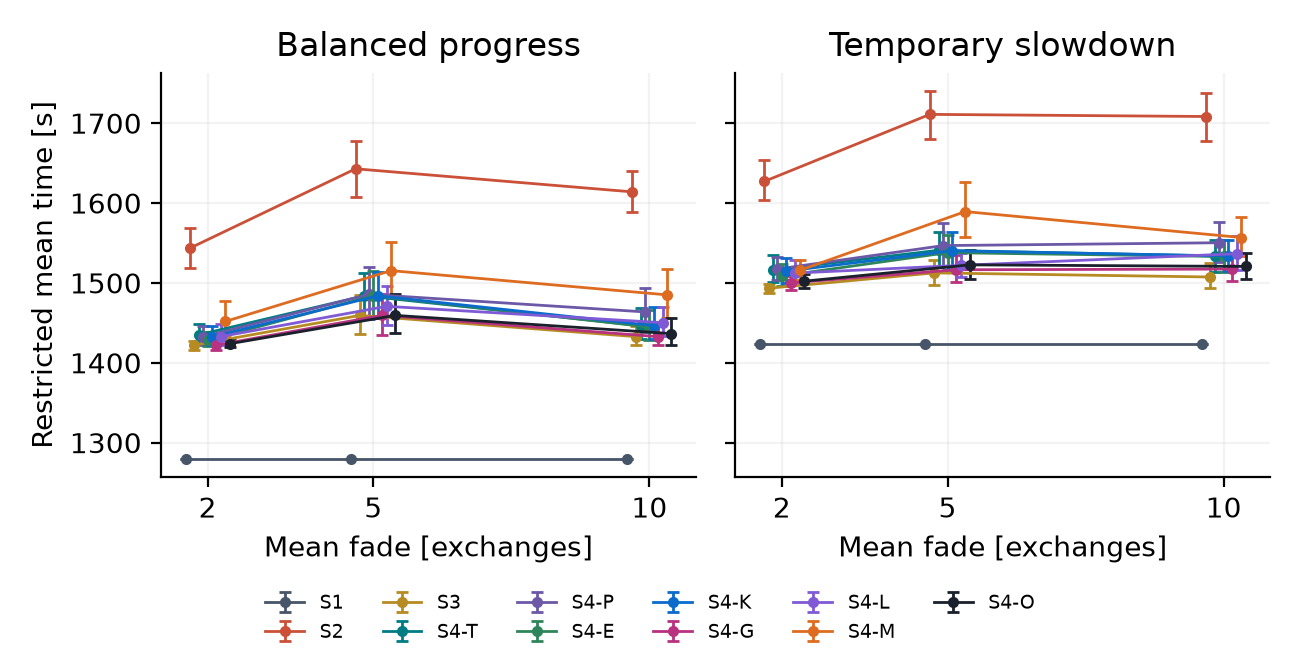
\includegraphics[width=\linewidth]{generated/extension/extension-mission-time.png}
\caption{Extension restricted mean time with 95\% paired-seed bootstrap intervals; markers are offset horizontally for legibility.}\label{fig:ext-time}\end{figure}
\begin{table}[htbp]\centering\scriptsize
\caption{Extension paired contrasts (B balanced, U unequal progress; negative favours the first policy). Marginal 95\% intervals from 2000 whole-seed resamples (seed 20261027).}\label{tab:ext-contrasts}
\begin{tabular}{llrrr}\toprule
Contrast & Condition & Mean [s] & 95\% CI [s] & Rel. [\%]\\\midrule
S4-T minus S2 & B, L=2 & -108 & [-137, -83] & -7.0\\
S4-T minus S3 & B, L=2 & 13 & [2, 26] & 0.9\\
S4-T minus S4-P & B, L=2 & 2 & [0, 8] & 0.2\\
S4-G minus S3 & B, L=2 & 0 & [0, 0] & 0.0\\
S4-O minus S3 & B, L=2 & 2 & [0, 4] & 0.1\\
S4-T minus S2 & B, L=5 & -159 & [-198, -122] & -9.7\\
S4-T minus S3 & B, L=5 & 24 & [5, 47] & 1.7\\
S4-T minus S4-P & B, L=5 & -2 & [-17, 11] & -0.1\\
S4-G minus S3 & B, L=5 & 0 & [0, 0] & 0.0\\
S4-O minus S3 & B, L=5 & 0 & [0, 0] & 0.0\\
S4-T minus S2 & B, L=10 & -168 & [-197, -140] & -10.4\\
S4-T minus S3 & B, L=10 & 14 & [1, 34] & 1.0\\
S4-T minus S4-P & B, L=10 & -17 & [-37, -2] & -1.2\\
S4-G minus S3 & B, L=10 & 0 & [0, 0] & 0.0\\
S4-O minus S3 & B, L=10 & 4 & [-4, 14] & 0.3\\
S4-T minus S2 & U, L=2 & -111 & [-137, -83] & -6.8\\
S4-T minus S3 & U, L=2 & 23 & [9, 41] & 1.5\\
S4-T minus S4-P & U, L=2 & -1 & [-9, 9] & -0.1\\
S4-G minus S3 & U, L=2 & 7 & [0, 15] & 0.4\\
S4-O minus S3 & U, L=2 & 9 & [2, 17] & 0.6\\
S4-T minus S2 & U, L=5 & -170 & [-201, -141] & -9.9\\
S4-T minus S3 & U, L=5 & 28 & [6, 52] & 1.9\\
S4-T minus S4-P & U, L=5 & -6 & [-21, 6] & -0.4\\
S4-G minus S3 & U, L=5 & 4 & [-4, 13] & 0.3\\
S4-O minus S3 & U, L=5 & 10 & [-1, 24] & 0.7\\
S4-T minus S2 & U, L=10 & -175 & [-208, -144] & -10.2\\
S4-T minus S3 & U, L=10 & 26 & [13, 43] & 1.7\\
S4-T minus S4-P & U, L=10 & -17 & [-32, -3] & -1.1\\
S4-G minus S3 & U, L=10 & 10 & [2, 19] & 0.7\\
S4-O minus S3 & U, L=10 & 13 & [5, 23] & 0.9\\
\bottomrule\end{tabular}

\end{table}

\paragraph{Hardware projection.} The work counted per decision is mapped to cycles under stated ranges. Software-emulated binary64 on the Cortex-M4F is assumed to take 20--100 cycles per operation and 200--1000 per transcendental call. The Cortex-M7 is assumed to take 1--4 and 40--150, and the Cortex-A72/A57 0.5--2 and 20--80. Clocks and RAM are nominal datasheet values. Board powers of 3.4 W (Raspberry Pi 4) and 10 W (Jetson Nano) follow \cite{niu2020depth} and are used only for order-of-magnitude comparison. The projection excludes caches, interpreter overhead, the radio and propulsion. It is not a measurement.
\begin{table}[htbp]\centering\scriptsize
\caption{Projected latency per warning decision [µs], low--high assumption range.}
\resizebox{\linewidth}{!}{\begin{tabular}{lrrrr}\toprule
Predictor & Cortex-M4F MCU & Cortex-M7 MCU & Raspberry Pi 4 & Jetson Nano CPU\\\midrule
Trend (frozen) & 31.1--155.3 & 1.3--5.1 & 0.2--0.9 & 0.2--0.9\\
Persistence (frozen) & 0.1--0.6 & 0.0--0.0 & 0.0--0.0 & 0.0--0.0\\
EWMA residual & 17.9--89.5 & 0.9--3.3 & 0.1--0.6 & 0.1--0.6\\
Kalman level/slope & 22.9--114.3 & 1.0--3.7 & 0.2--0.6 & 0.2--0.6\\
Gilbert burst HMM & 43.5--213.8 & 1.7--5.8 & 0.3--1.0 & 0.3--1.0\\
Logistic regression & 27.0--134.7 & 1.2--4.4 & 0.2--0.7 & 0.2--0.8\\
MLP (16 tanh) & 82.0--409.7 & 3.1--11.9 & 0.5--2.0 & 0.5--2.1\\
Fade oracle (bound) & 15.8--78.8 & 0.8--3.0 & 0.1--0.5 & 0.1--0.5\\
\bottomrule\end{tabular}
}
\end{table}

\paragraph{Map-accuracy diagnostic.} The seabed is a plane (18 m plus a 0.04 slope eastward) with 24 random cosine modes (wavelengths 40--220 m) and 0.4 m sand waves. All soundings use binary64, and noise streams are seeded per run. Checkpoints every 300 s give a common time axis; after stopping, the map is held fixed. RMSE covers all 24\,000 sounding locations, including interpolated unobserved cells. The S-44 fraction counts locations whose absolute error is within the Order 1a TVU.
\begin{table}[htbp]\centering\scriptsize
\caption{Synthetic map accuracy per policy (core: 180 frozen runs each; extension: 180 runs each). The last column counts runs reaching 0.5 m RMSE before timeout.}
\begin{tabular}{llrrrrr}\toprule
Study & Policy & RMSE 900 s & RMSE 1800 s & Final RMSE & S-44 1a [\%] & $\le$0.5 m runs\\\midrule
core & S1 & 1.52 & 0.35 & 0.35 & 91.8 & 180/180\\
core & S2 & 2.50 & 2.50 & 2.50 & 34.3 & 0/180\\
core & S3 & 1.31 & 0.57 & 0.57 & 85.7 & 158/180\\
core & S4-T & 1.33 & 0.60 & 0.60 & 85.0 & 156/180\\
core & S4-P & 1.29 & 0.54 & 0.53 & 86.9 & 162/180\\
extension & S1 & 1.52 & 0.35 & 0.35 & 91.7 & 180/180\\
extension & S2 & 1.46 & 0.33 & 0.33 & 93.0 & 180/180\\
extension & S3 & 1.16 & 0.34 & 0.34 & 92.3 & 180/180\\
extension & S4-T & 1.17 & 0.34 & 0.34 & 92.4 & 180/180\\
extension & S4-P & 1.16 & 0.34 & 0.34 & 92.5 & 180/180\\
extension & S4-E & 1.15 & 0.34 & 0.34 & 92.4 & 180/180\\
extension & S4-K & 1.17 & 0.34 & 0.34 & 92.4 & 180/180\\
extension & S4-G & 1.16 & 0.34 & 0.34 & 92.3 & 180/180\\
extension & S4-L & 1.14 & 0.34 & 0.34 & 92.4 & 180/180\\
extension & S4-M & 1.17 & 0.34 & 0.34 & 92.5 & 180/180\\
extension & S4-O & 1.16 & 0.34 & 0.34 & 92.4 & 180/180\\
\bottomrule\end{tabular}

\end{table}
